\chapter{Технологический раздел}
\label{cha:implementation}

\section{Формат описания модели объектно-ориентированной программы}

Основой является формат YAML~\cite{YAML}.
Формат был выбран благодаря следующим достоинствам:
\begin{itemize}
\item текстовое представление;
\item поддержка рекурсивных структур и ссылок;
\item поддержка пользовательских типов данных.
\end{itemize}

Корневой элемент модели помечается тегом \verb;!Model; и является списком элементов
модели:
\begin{minted}{yaml}
!Model:
- <Classifier>
\end{minted}

\verb;Classifier; -- любой из элементов, помеченный тегом \verb;!Class;,
\verb;!Classifier;, \verb;!Interface;, \verb;!PrimitiveType;,
который имеет структуру:
\begin{minted}{yaml}
!Classifier
name: <str>
properties:
  - <Property>
operations:
  - <Operation>
generals:
  - <Classifier>
suppliers:
  - <Classifier>
\end{minted}

Каждый из атрибутов является опциональным.
Если не задано имя (\verb;name;), то элементу будет задано уникальное
имя вида \verb;anonymous_<число>;.
Выполняется для такого же атрибута других типов элементов.

\verb;Property; --- элемент, помеченный тегом \verb;!Property; со следующей
структурой:
\begin{minted}{yaml}
!Property
name: <str>
type: <Type>
visibility: <Visibility>
aggregation: <Aggregation>
is_static: <bool>
owner: <Classifier>
\end{minted}

\verb;Operation; --- элемент, помеченный тегом \verb;!Operation; со следующей
структурой:
\begin{minted}{yaml}
!Operation
name: <str>
result: <Type>
visibility: <Visibility>
parameters:
  - <Parameter>
is_static: <bool>
invocations:
  - <Operation>
owner: <Classifier>
\end{minted}

\verb;Type; --- элемент, помеченный тегом \verb;!Type; со следующей
структурой:
\begin{minted}{yaml}
!Operation
classifier: <Classifier>
lower: <int>
upper: <int>
is_ordered: <bool>
is_unique: <bool>
\end{minted}

\verb;Visibility; --- элемент, помеченный тегом \verb;!Visibility;,
имеющий одно из допустимых значений:
\begin{itemize}
\item \verb;'public';
\item \verb;'protected';
\item \verb;'private';
\end{itemize}

\verb;Aggregation; --- элемент, помеченный тегом \verb;!Aggregation;,
имеющий одно из допустимых значений:
\begin{itemize}
\item \verb;'none';
\item \verb;'shared';
\item \verb;'composite';
\end{itemize}

\textbf{YAML} предоставляет возможность ссылаться на другие элементы по адресу.
Каждый элемент должен быть описан один раз.
Например, если нужно описать связь наследования между двумя классами, можно
сделать следующим образом:
\begin{minted}{yaml}
!Model
- &id001 !Class
  name: Base
- !Class
  name: Derived
  generals:
  - *id001
\end{minted}

\verb;&id001; означает, что классу с названием \verb;Base; присваивается такой
адрес. В перечислении базовых классов в классе с названием \verb;Derived;
указывается ссылка \verb;*id001; на \verb;Base;.

\section{Структура программного комлекса}

Для реализации разработанного метода разработан программный комплекс,
который позволяет выполнять поиск шаблонов проектирования в программах,
написанных на языке программирования \textbf{Java}.

В комплекс входят следующие программы:
\begin{itemize}
\item \textbf{java\_source\_model} --- программа для построения модели программы
на языке Java;
\item \textbf{java\_bytecode\_model} --- программа для построения модели программы
на основе байткода для виртуальной машины \textbf{Java};
\item \textbf{pattern\_model} --- программа для построения модели шаблона;
\item \textbf{match\_pattern} --- программа для поиска шаблонов проектирования.
\end{itemize}

Основной сценарий использования программного комплекса:
\begin{enumerate}
\item построение модели программы с помощью \textbf{java\_source\_model} или \textbf{java\_bytecode\_model};
\item построение модели шаблона из заранее заготовленных с помощью \textbf{pattern\_model};
\item запуск \textbf{match\_pattern} с результатами первых двух шагов в качестве входных данных.
\end{enumerate}

Модель программы или шаблона можно описать вручную.

Программы \textbf{java\_source\_model}, \textbf{pattern\_model},
\textbf{match\_pattern} написаны на языке \textbf{Python} версии 2.7.
\textbf{java\_bytecode\_model} написана на \textbf{Java} версии 1.8.

Структура компонентов и зависимостей программного комплекса представлена на
рисунке~\ref{fig:components}.

\begin{figure}[!ht]
\centering
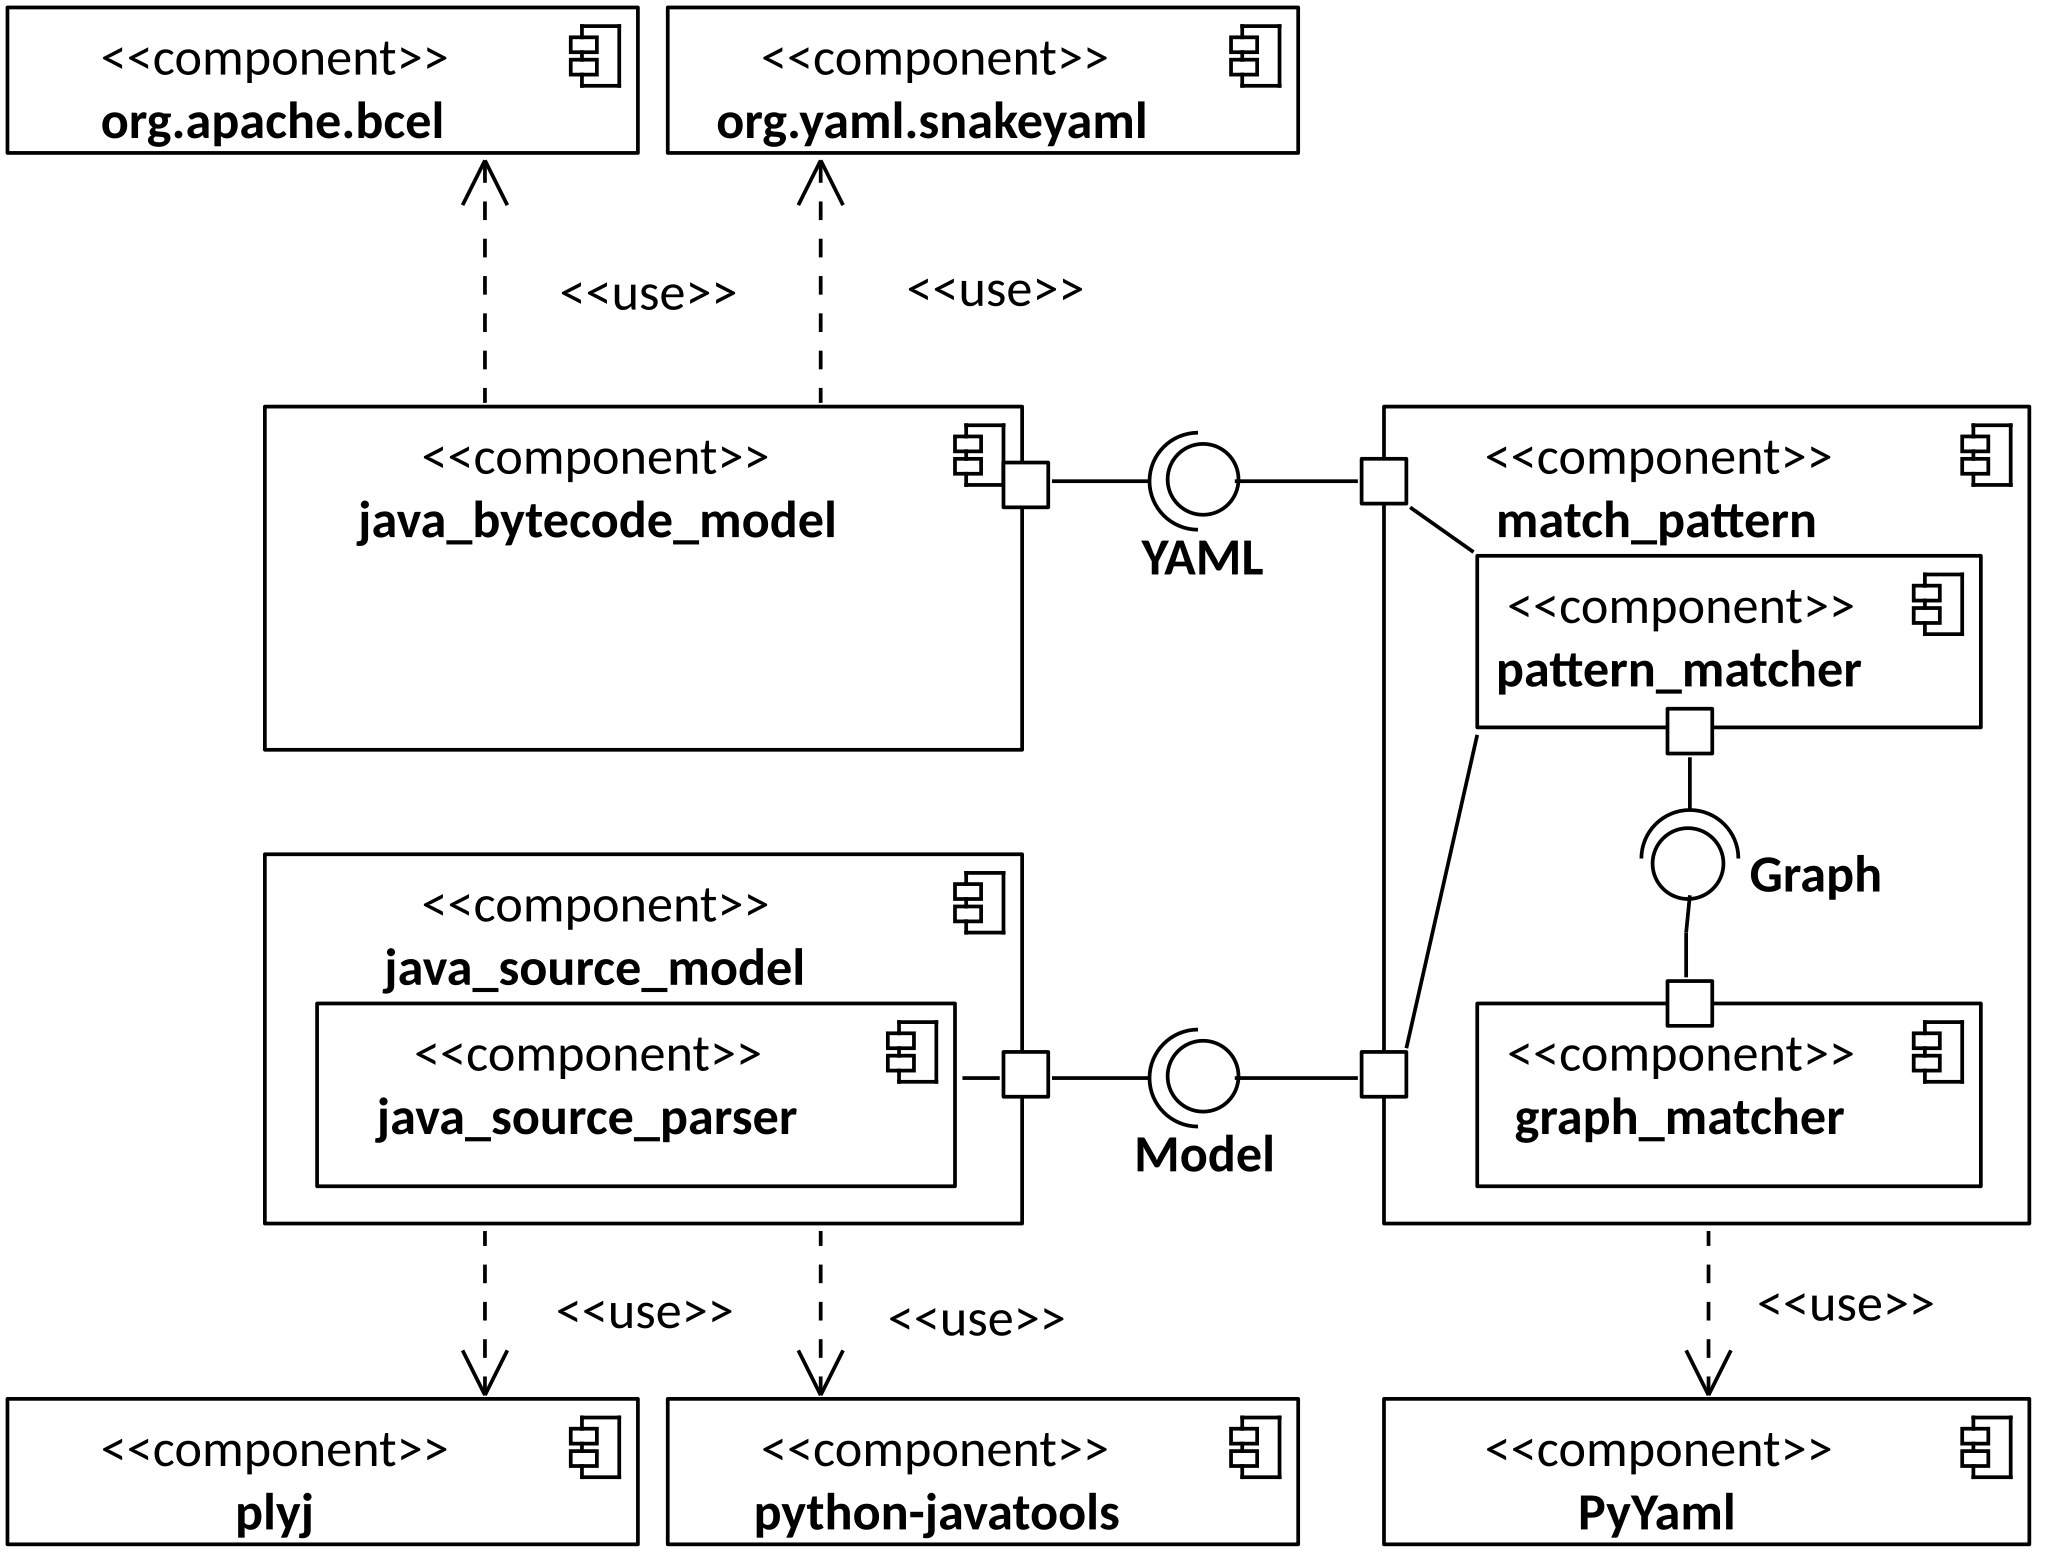
\includegraphics[width=\textwidth]{inc/components.pdf}
\caption{Структура компонентов и зависимостей программного комплекса}
\label{fig:components}
\end{figure}

\subsection{Программа для построения модели программы на языке Java}

Выполняет синтаксический анализ исходного кода на языке \textbf{Java} с выводом
полных имен типов.
Программа может работать с одним или множество файлов формата \textbf{.java}.
Для синтаксического анализа используется библиотека \textbf{plyj}~\cite{plyj}.
Определение полных имен внешних типов выполняется с помошью \textbf{.class} или
\textbf{.jar}-файлов.
Для их анализа используется библиотека \textbf{javatools}~\cite{javatools}.
Вывод модели в формате \textbf{.yaml} выполняется с помощью библиотеки
\textbf{PyYAML}~\cite{PyYAML}.

Интерфейс запуска:
\begin{verbatim}
python java_source_model.py [-h] [-p <external_path>] <path> [<path> ...]
\end{verbatim}

\begin{itemize}
\item \verb;path; --- путь к .java файлу или директории;
\item \verb;-h; или \verb;--help; --- выводит сообщение с описанием параметров
запуска;
\item \verb;-p <external_path>; или \verb;--path <external_path>; --- задает
путь \verb;external_path; к \textbf{.class}, \textbf{.jar} файлам или директории;
\end{itemize}

Выводит модель в формате \textbf{.yaml} в \textbf{stdout}.
Сообщения об ошибках выводятся в \textbf{stderr}.

Алгоритм работы программы:
\begin{enumerate}
\item рекурсивно найти все \textbf{.java}-файлы по всем заданным путям;
\item выполнить синтаксический анализ всех \textbf{.java}-файлов и построить
деревья вывода;
\item во всех деревьях вывода установить полные имена классов в их определении.
\item создать пустые элементы модели: классы, интерфейсы и перечисления;
\item создать пустые элементы модели для внешних зависимостей;
\item во всех деревьях вывода установить полные имена типов в любых местах их
использования;
\item определить связи обобщения;
\item заполнить элементы модели свойствами, операциями и создать типы данных;
\item определить связи зависимости;
\item вывести модель в формате \textbf{.yaml}.
\end{enumerate}

При анализе программ с множеством пакетов и вложенных классов может возникнуть
ситуация конфликта имен.
Допустим \verb;class A; есть в \verb;package x; и в \verb;package y;.
Это два разных класса.
В исходном коде и дереве вывода скорее всего будет представлено короткое название
для каждого класса.
При построении модели недопустимо использовать эти короткие названия.
Нужно вывести полное названия типа.
Таким образом, в модель попадут классы \verb;x.A; и \verb;y.A;.
В этом случае конфликта имен не будет.

Проблема имеет место не только в определениях типов, но и в их использовании.
Например, есть \verb;class x.A;, \verb;class y.A; и в \verb;class z.B; определен
метод \verb;A f();.
Нужно определить полное имя возвращаемого типа.
Сюда же можно отнести определение типа поля класса, локальной переменной,
параметра метода, базового класса.
В данном случае нужно учитывать, импорт какого пакета был выполнен.
Аналогичная ситуация с вложенными классами.

Другая проблема, которая не решалась в этой программе, заключается в определении
зависимостей между вызываемым и вызывающим методов.

Программа не во всех случая определяет полные имена типов.
В таких случая классы, интефейсы и перечисления их представляющие игнорируются
при построении модели.
Здесь не будут описаны все ситуации, когда тип определяется, а когда нет.
Разработка программы была приостановлена.
Для дальнейшей разработки требовалось написание части компилятора \textbf{Java}.
Реальной необходимости в этом не было
поэтому взамен была написана программа на \textbf{Java},
которая содержит всю нужную функциональность.
Она описана в следующем разделе.

\subsection{Программа для построения модели программы на основе байткода для виртуальной машины Java}

Анализирует байткод виртуальной машины \textbf{Java}.
Для этого используется библиотека \textbf{Apache Commons BCEL}
(The Byte Code Engineering Library) версии 6.0~\cite{BCEL}.
Для сборки программы используется \textbf{Apache Maven} версии 3~\cite{Maven}.

Интерфейс запуска:
\begin{verbatim}
java -jar java_bytecode_model.jar <path> [<path> ...]
\end{verbatim}

\begin{itemize}
\item \verb;path; --- путь к \textbf{.class}, \textbf{.jar}-файлу или директории;
\end{itemize}

Выводит модель в формате \textbf{.yaml} в \textbf{stdout}.
Сообщения об ошибках выводятся в \textbf{stderr}.

Алгоритм работы программы:
\begin{enumerate}
\item рекурсивно и разобрать найти все \textbf{.jar} и \textbf{.class}-файлы по
всем заданным путям, \textbf{.class}-файлы в \textbf{.jar}-файлах;
\item создать пустые элементы модели для классов, интерфейсов и перечислений;
\item определить связи -- обобщения;
\item создать типы данных;
\item заполнить элементы модели свойствами и операциями;
\item определить связи -- зависимости;
\item определить связи -- вызовы методов;
\item вывести модель в формате \textbf{.yaml}.
\end{enumerate}

\subsection{Программа для построения модели шаблона}

Строит модель для одного из заготовленных шаблонов.

Интерфейс запуска:
\begin{verbatim}
python pattern_model.py [-h] <name>
\end{verbatim}

\begin{itemize}
\item \verb;name; --- название шаблона проектирования;
\item \verb;-h; или \verb;--help; --- выводит сообщение с описанием параметров
запуска.
\end{itemize}

Выводит модель в формате \textbf{.yaml} в \textbf{stdout}.
Сообщения об ошибках выводятся в \textbf{stderr}.

Реализованы следующие шаблоны:
\begin{itemize}
\item \textbf{AbstractFactory} --- абстрактная фабрика;
\item \textbf{BaseDerived} --- связка базового и производного классов;
\item \textbf{Bridge} --- мост;
\item \textbf{ChainOfResponsibility} --- цепочка ответственности;
\item \textbf{Decorator} --- декоратор;
\item \textbf{Empty} --- пустой, используется для тестирования;
\item \textbf{Memento} --- хранитель;
\item \textbf{OverriddenMethodCall} --- вызов метода базового класса,
переопределеного в производном;
\item \textbf{Visitor} --- посетитель.
\end{itemize}

\subsection{Программа для поиска шаблонов проектирования}

Выполняет поиск изоморфизмов между моделями объектно-ориетированных систем.
Для чтения модели используется библиотека \textbf{PyYAML}.

Интерфейс запуска:
\begin{verbatim}
python match_pattern.py [-h] [-l <limit>] [-v <level>] <pattern> <target>
\end{verbatim}

\begin{itemize}
\item \verb;pattern; --- путь к \textbf{.yaml}-файлу модели шаблона;
\item \verb;target; --- путь к \textbf{.yaml}-файлу целевой модели;
\item \verb;-h; или \verb;--help; --- выводит сообщение с описанием параметров
запуска;
\item \verb;-l <limit>; или \verb;--limit <limit>; --- задает максимальное
количество изоморфизмов \verb;limit;, которое нужно найти;
в наибольшей;
\item \verb;-v <level>; или \verb;--verbosity <level>; --- включает вывод
журнала в \textbf{stderr} с уровнем подробности \verb;level;:
\begin{itemize}
\item \verb;DEBUG; --- подробный отладочный вывод;
\item \verb;INFO; --- выводится основная информация.
\end{itemize}
\end{itemize}

Выводит варианты соответствий элементов в \textbf{stdout}.
Сообщения об ошибках выводятся в \textbf{stderr}.

\subsubsection{Модуль graph\_matcher}

В этом модуле реализован алгоритм поиска изоморфного подграфа.
Структура классов представлена на рисунке~\ref{fig:graph-matcher}.

\begin{figure}[!ht]
\centering
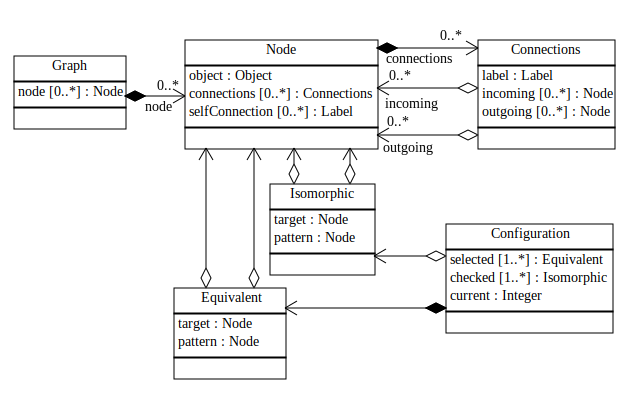
\includegraphics[width=\textwidth]{inc/graph-matcher.pdf}
\caption{Структура классов модуля graph\_matcher}
\label{fig:graph-matcher}
\end{figure}

\textbf{Graph} --- граф.

Атрибуты:
\begin{itemize}
\item \textbf{node} --- множество вершин;
\end{itemize}

\textbf{Node} --- вершина графа.

Атрибуты:
\begin{itemize}
\item \textbf{object} --- значение вершины;
\item \textbf{connections} --- множество множеств дуг одного типа;
\item \textbf{selfConnection} --- множество типов дуг, которые соединяют вершину саму с собой;
\end{itemize}

\textbf{Connections} --- множество дуг одного типа.

Атрибуты:
\begin{itemize}
\item \textbf{label} --- метка дуг;
\item \textbf{incoming} --- множество вершин, в которые входят дуги, исходящие из текущей вершины;
\item \textbf{selfConnection} --- множество вершин, из которых исходят дуги, входящие в текущую вершины.
\end{itemize}

\textbf{Equivalent} --- пара эквивалентных вершин.

Атрибуты:
\begin{itemize}
\item \textbf{target} --- вершина целевого графа;
\item \textbf{pattern} --- вершина шаблона.
\end{itemize}

\textbf{Isomoprhic} --- пара изоморфных вершин.

Атрибуты:
\begin{itemize}
\item \textbf{target} --- вершина целевого графа;
\item \textbf{pattern} --- вершина шаблона.
\end{itemize}

\textbf{Configuration} --- конфигурация алгоритма поиска изоморфного подграфа.

Атрибуты:
\begin{itemize}
\item \textbf{selected} --- последовательность пар вершин, которые нужно проверить;
\item \textbf{checked} --- множество изоморфных вершин;
\item \textbf{current} --- индекс текущей вершины в последовательности \textbf{selected}.
\end{itemize}

Реализация алгоритма поиска изоморфных подграфов --- функция \textbf{match}:

\begin{minted}{python}
def match(target_graph, pattern_graph, match_largest_target_component=False)
\end{minted}

Параметры:
\begin{itemize}
\item \textbf{target\_graph} --- целевой граф, объект типа \textbf{Graph};
\item \textbf{pattern\_graph} --- граф шаблона, объект типа \textbf{Graph};
\end{itemize}

Возвращает генератор списков объектов типа \textbf{Isomoprhic}.

Здесь же реализована проверка результата алгоритма --- функция \textbf{check}:

\begin{minted}{python}
def check(isomorphism)
\end{minted}

\textbf{isomorphism} --- коллекция или генератор объектов типа \textbf{Isomoprhic}.

\subsubsection{Модуль pattern\_matcher}

В этом модуле реализован алгоритм поиска шаблона проектирования в модели
объектно-ориентированной системы.
Структура связей обобщения классов представлена на рисунке~\ref{fig:pattern-matcher-generalizations}.
Структура ассоциаций классов представлена на рисунке~\ref{fig:pattern-matcher-associations}.

\begin{figure}[!ht]
\centering
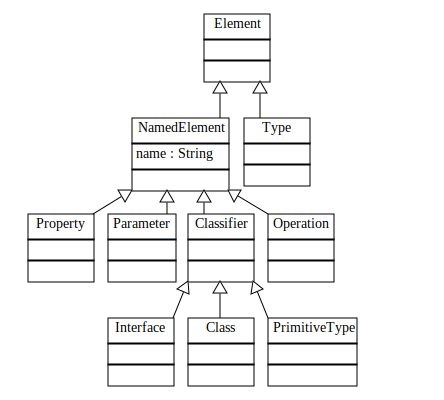
\includegraphics{inc/pattern-matcher-generalizations.pdf}
\caption{Структура классов модуля pattern\_matcher. Обобщения}
\label{fig:pattern-matcher-generalizations}
\end{figure}

\begin{figure}[!ht]
\centering
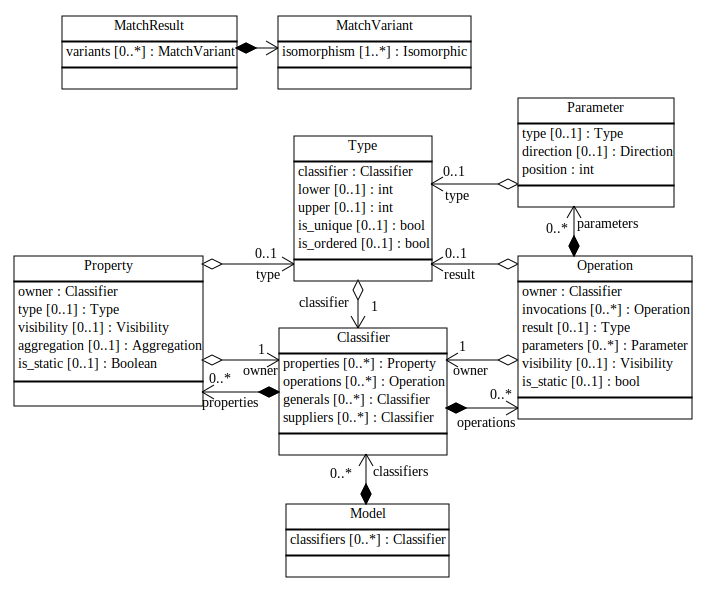
\includegraphics[width=\textwidth]{inc/pattern-matcher-associations.pdf}
\caption{Структура классов модуля pattern\_matcher. Ассоциации}
\label{fig:pattern-matcher-associations}
\end{figure}

\textbf{Element} --- базовый элемент модели.

\textbf{NamedElement} --- именованный элемент модели.

Атрибуты:
\begin{itemize}
\item \textbf{name} --- название, уникальное в зависимости от контекста.
\end{itemize}

\textbf{Aggregation} --- тип агрегации для свойства.

Допустимые значения:
\begin{itemize}
\item \textbf{none} --- отсутствует;
\item \textbf{shared} --- классификатор ссылается на объект;
\item \textbf{composite} --- классификатор владеет объектом;
\end{itemize}

\textbf{Direction} --- тип параметра метода.

Допустимые значения:
\begin{itemize}
\item \textbf{in} --- метод только читает значение параметра и может изменять его состояние;
\item \textbf{out} --- метод только изменяет значение параметра;
\item \textbf{inout} --- метод читает и изменяет значение параметра;
\end{itemize}

\textbf{Visibility} --- доступность свойства или метода, допустимые значения.

Атрибуты:
\begin{itemize}
\item \textbf{private} --- только из этого же классификатора;
\item \textbf{protected} --- из этого класса и всех производных классификаторов;
\item \textbf{public} --- из любого места;
\end{itemize}

\textbf{Classifier} --- классификатор.

Атрибуты:
\begin{itemize}
\item \textbf{name} --- имя, уникальное для модели;
\item \textbf{poperty} --- свойства классификатора;
\item \textbf{operation} --- операции классификатора;
\item \textbf{general} --- базовые классификаторы;
\item \textbf{suppliers} --- используемые классификаторы;
\end{itemize}

\textbf{Property} --- свойство классификатора.

Атрибуты:
\begin{itemize}
\item \textbf{name} --- имя, уникальное для классификатора;
\item \textbf{owner} --- класс, которому принадлежит свойство;
\item \textbf{type} --- тип свойства;
\item \textbf{visibility} --- доступность;
\item \textbf{is\_static} --- имеет ли свойство одно значение для всех объектов классификатора;
\end{itemize}

\textbf{Operation} --- операция классификатора.
Атрибуты:
\begin{itemize}
\item \textbf{name} --- имя, уникальное для классификатора, типа результата и списка типов параметров;
\item \textbf{owner} --- классификатора, которому принадлежит операция;
\item \textbf{invoke} --- вызываемые операции;
\item \textbf{result} --- тип результата;
\item \textbf{parameter} --- список параметров;
\item \textbf{visibility} --- доступность;
\item \textbf{is\_static} --- запрещено ли методу оперировать состоянием объекта;
\end{itemize}

\textbf{Parameter} --- параметр метода класса.

Атрибуты:
\begin{itemize}
\item \textbf{name} --- имя, уникальное для операции;
\item \textbf{type} --- тип значения;
\item \textbf{direction} --- тип параметра;
\item \textbf{position} --- порядковый номер;
\end{itemize}

\textbf{Type} --- любой тип данных.

Атрибуты:
\begin{itemize}
\item \textbf{classifier} --- классификатор типа;
\item \textbf{lower} --- нижняя граница множественности $\left [ 0, upper \right ]$;
\item \textbf{upper} --- верхняя граница множественности $\left [ lower, \infty \right ]$;
\item \textbf{is\_unique} --- должны ли значения быть уникальными, если есть множественность;
\item \textbf{is\_ordered} --- упорядочены ли значения, если есть множественность.
\end{itemize}

\textbf{Class} --- класс.

\textbf{Interface} --- интерфейс.

\textbf{PrimitiveType} --- примитивный тип данных, например \textbf{int} в \textbf{Java}.

\textbf{Model} --- модель объектно-ориентированной системы.

\textbf{MatchResult} --- результат поиска шаблонов проектирования.

\textbf{MatchVariant} --- вариант соответствия элементов цели элементам шаблона.

Атрибуты:
\begin{itemize}
\item \textbf{isomorphic} --- кортеж (\textbf{tuple}) пар объектов типа \textbf{Element}.
\end{itemize}

Реализация алгоритма поиска шаблонов проектирования --- функция \textbf{match}:

\begin{minted}{python}
def match(target, pattern, limit=None)
\end{minted}

Параметры:
\begin{itemize}
\item \textbf{target} --- целевая модель, объект типа \textbf{Model};
\item \textbf{pattern} --- модель шаблона, объект типа \textbf{Model};
\item \textbf{limit} --- \textbf{int}, максимальное количество
вариантов, которое нужно найти. Если \textbf{None}, то выполняется поиск всех;
\end{itemize}

\section{Тестирование}

Все тесты написаны на языке Python.
Для запуска используется фреймворк \textbf{pytest}~\cite{pytest}.

\subsection{Модульное тестирование}

Для написания модульных тестов использовались библиотеки:
\begin{itemize}
\item \textbf{unittest} --- для описания структуры тестов;
\item \textbf{PyHamcrest}~\cite{PyHamcrest} --- для описания проверок в тестах.
\end{itemize}

\subsubsection{Тестирование модуля graph\_matcher}

Протестировано создание объектов классов и их состояния:
\begin{itemize}
\item \textbf{Node};
\item \textbf{Configuration};
\item \textbf{Equivalent};
\item \textbf{Isomorphic};
\item \textbf{Graph}.
\end{itemize}

Функций:
\begin{itemize}
\item \textbf{Graph.get\_connected\_cmponents} --- реализация алгоритма поиска
компонент связности графа;
\item \textbf{match} --- реализация алгоритма поиска изоморфных подграфов.
\end{itemize}

Цель --- проверить простейшие ситуации на графах из нескольких вершин.
Для этого написаны тесты, представленные в таблице~\ref{table:match-graph-tests}.

\begin{table}[ht!]
    \centering
    \begin{tabulary}{\textwidth}{|C|C|C|C|}
        \hline
        № & Целевой граф & Граф шаблона & Результат \\
        \hline
        1 & $(\varnothing, \varnothing, \varnothing)$ & $(\varnothing, \varnothing, \varnothing)$ & $\varnothing$ \\
        \hline
        2 & $(\{ 1 \}, \varnothing, \varnothing)$ & $(\{ a \}, \varnothing, \varnothing)$ & $\{ (1, a) \}$ \\
        \hline
        3 & $(\{ 1, 2 \}, \varnothing, \varnothing)$ & $(\{ a \}, \varnothing, \varnothing)$ & $\{ (1, a) \}$, $\{ (2, a) \}$ \\
        \hline
        4 & $(\{ 1 \}, \varnothing, \varnothing)$ & $(\{ a, b \}, \varnothing, \varnothing)$ & $\{ (1, a) \}$, $\{ (1, b) \}$ \\
        \hline
        5 & $(\{ 1, 2 \}$, $\{ l \}$, $\{ ( 1, 2, l ) \})$ & $(\{ a, b \}$, $\{ l \}$, $\{ ( a, b, l ) \})$ & $\{ (1, a), (2, b) \}$ \\
        \hline
        6 & $(\{ 1, 2 \}$, $\{ x \}$, $\{ ( 1, 2, x ) \})$ & $(\{ a, b \}$, $\{ y \}$, $\{ ( a, b, y ) \})$ & $\varnothing$ \\
        \hline
        7 & $(\{ 1 \}$, $\{ l \}$, $\{ ( 1, 1, l ) \})$ & $(\{ a \}, \{ l \}$, $\{ ( a, a, l ) \})$ & $\{ (1, a) \}$ \\
        \hline
        8 & $(\{ 1, 2, 3 \}$, $\{ l \}$, $\{ ( 1, 2, l ), ( 2, 3, l ) \})$ & $(\{ a, b \}$, $\{ l \}$, $\{ ( a, b, l ), ( b, a, l ) \})$ & $\varnothing$ \\
        \hline
        9 & $(\{ 1, 2, 3 \}$, $\{ l \}$, $\{ ( 1, 2, l ), ( 2, 3, l ) \})$ & $(\{ a, b \}$, $\{ l \}$, $\{ ( a, b, l ) \})$ & $\{ (1, a), (2, b) \}$, $\{ (2, a), (3, b) \}$ \\
        \hline
        10 & $(\{ 1, 2, 3, 4 \}$, $\{ l \}$, $\{ ( 1, 2, l ), ( 3, 4, l ) \})$ & $(\{ a, b \}$, $\{ l \}$ , $\{ ( a, b, l ) \})$ & $\{ (1, a), (2, b) \}$, $\{ (3, a), (4, b) \}$ \\
        \hline
    \end{tabulary}
    \caption{Простейшие тесты алгоритма поиска изоморфных подграфов}
    \label{table:match-graph-tests}
\end{table}

Также протестированы случаи:
\begin{itemize}
\item у вершин заданы функции эквивалентности;
\item полные графы из четырех вершин;
\item все возможные графы из 2-4 вершин;
\end{itemize}

В случае со всеми возможными графами из 2, 3, 4 вершин применяется следующий алгоритм:

\begin{algorithmic}
\ForAll{ $n \in \{ 2, 3, 4 \}$ }
    \ForAll{ $G_t \in$ множество всех возможных графов из одной компоненты}
        \ForAll{ $G_p = (V_p, L_p, E_p) \in$ множество всех возможных подграфов $G_t$}
            \ForAll{ $I \in$ \Call{match}{$G_t$, $G_p$}}
                \State \Call{assert}{\Call{check}{$I$}}
                \State $V^I_p \gets \{ v_p : (v_t, v_p) \in I \}$
                \State \Call{assert}{$V_p = V^I_p$}
            \EndFor
        \EndFor
    \EndFor
\EndFor
\State \Return $C$
\end{algorithmic}

Тестирование для большего количества вершин требует неприемлимо большого
количества времени.

В процессе разработки были найдены ошибки, часть из которых была исправлена,
и для которых были написаны тесты:
\begin{itemize}
\item выполнение проверки на изоморфизм графов, состоящих из вершин,
которые находятся в множестве $checked$ конфигурации алгоритма;
\item поиск изоморфного подграфа из двух компонент, имеющих по одной дуге,
в графе из одной компоненты, имеющей несколько дуг.
\end{itemize}

В первом случае ошибка проявлялась на графах, представленных на
рисунках \ref{fig:check-current-isomorphism-target}
\ref{fig:check-current-isomorphism-pattern}.

\begin{figure}[!ht]
\centering
\includegraphics{inc/check-current-isomorphism-target.pdf}
\caption{Целевой граф}
\label{fig:check-current-isomorphism-target}
\end{figure}

\begin{figure}[!ht]
\centering
\includegraphics{inc/check-current-isomorphism-pattern.pdf}
\caption{Граф шаблона}
\label{fig:check-current-isomorphism-pattern}
\end{figure}

Ожидался следующий результат:
\begin{itemize}
\item $\{ (1, a), (2, e), (3, b), (4, c), (6, d) \}$
\item $\{ (1, a), (3, b), (4, c), (5, e), (6, d) \}$
\item $\{ (1, a), (2, d), (3, c), (4, b), (6, e) \}$
\item $\{ (1, a), (3, c), (4, b), (5, d), (6, e) \}$
\end{itemize}
Первый вариант результат представлен на
рисунке~\ref{fig:check-current-isomorphism-result}.

\begin{figure}[!ht]
\centering
\includegraphics{inc/check-current-isomorphism-result.pdf}
\caption{Вариант изоморфизма графов}
\label{fig:check-current-isomorphism-result}
\end{figure}

Отсутсвие проверки приводило к дополнительным вариантам:
\begin{itemize}
\item $\{ (1, a), (2, e), (3, c), (4, b), (5, d) \}$
\item $\{ (1, a), (2, d), (3, b), (4, c), (5, e) \}$
\end{itemize}
Первый вариант представлен на
рисунке~\ref{fig:check-current-isomorphism-invalid-result}.
Здесь вершина $4 \cong b$ соединена с тремя вершинами шаблона,
что невозможно, так как вершина $b$ имеет только две связи.

\begin{figure}[!ht]
\centering
\includegraphics{inc/check-current-isomorphism-invalid-result.pdf}
\caption{Варианта ошибочного изоморфизма графов}
\label{fig:check-current-isomorphism-invalid-result}
\end{figure}

Во втором случае ошибка заключается в отсутствии объединения результатов.
Для графов $G_t = (\{ 1, 2, 3, 4 \}, \{ l \}, \{ (1, 2, l), (2, 3, l), (3, 4, l) \})$
и $G_p = (\{ a, b, c, d \}, \{ l \}, \{ (a, b, l), (c, d, l) \})$
результат должен быть таким:
$\{ (1, a), (2, b), (3, c), (4, d) \}$,
$\{ (2, a), (3, b) \}$,
$\{ (1, c), (2, d), (3, a), (4, b) \}$,
$\{ (2, c), (3, d) \}$;
но результат следующий:
$\{ (1, a), (2, b) \}$,
$\{ (2, a), (3, b) \}$,
$\{ (3, a), (4, b) \}$,
$\{ (1, c), (2, d) \}$,
$\{ (2, c), (3, d) \}$,
$\{ (3, c), (4, d) \}$.
Учитывая, что в данной работе не используются шаблоны из нескольких компонент
связности, можно исправить ошибку позднее, когда это потребуется.

Подробные результаты приведены в приложении~А.

\subsubsection{Тестирование модуля pattern\_matcher}

Протестировано создание объектов классов и их состояния:
\begin{itemize}
\item \textbf{Aggregation};
\item \textbf{Class};
\item \textbf{Classifier};
\item \textbf{Direction};
\item \textbf{Interface};
\item \textbf{Model};
\item \textbf{MatchVariant};
\item \textbf{MatchResult};
\item \textbf{Operation};
\item \textbf{Parameter};
\item \textbf{PrimitiveType};
\item \textbf{Property};
\item \textbf{Type};
\item \textbf{Visibility}.
\end{itemize}

Функций:
\begin{itemize}
\item \textbf{eq\_ignore\_order} --- сравнение коллекций без учета порядка;
\item \textbf{match} --- реализация алгоритма поиска шаблона проектирования в модели;
\item \textbf{check} --- проверка результата \textbf{match};
\item чтения и записи модели и отдельных ее элементов в формате \textbf{YAML}.
\end{itemize}

Подробные результаты приведены в приложении~В.

\subsection{Функциональное тестирование}

Здесь проверялась работа программ, использовались заранее подготовленные данные
и ожидаемые результаты в виде файлов.

\subsubsection{Тестирование программы java\_bytecode\_model}

В качестве входных данных используются \textbf{.java}-файлы.
Выполняется их компиляция и запуск \textbf{java\_bytecode\_model} с
получившимися \textbf{.class}-файлами.
Резульат выполнения программы сравнивается с заранее заготовленными
\textbf{.yaml}-файлами.

Проводятся следующие тесты создания модели для:
\begin{itemize}
\item пустого файла;
\item одного класса (\textbf{class});
\item одного перечисления (\textbf{enum});
\item одного интерфейса (\textbf{interface});
\item двух классов, связанных обобщением (\textbf{extends});
\item двух интерфейсов и класса, связанных обобщением (\textbf{implements});
\item иерархии обобщения из шести классов, на трех уровнях;
\item класса со свойствами;
\item класса с методами;
\item зависимостей между классами;
\item вызовов методов внутри класса и между классами;
\item вызова переопределенного метода.
\end{itemize}

Подробные результаты приведены в приложении~Г.

\subsubsection{Тестирование программы match\_pattern}

Для моделей, описанных в \textbf{.yaml}-файлах, выполняется поиск шаблонов,
реализованных в программе \textbf{pattern\_model}.
Результат сравнивается с записанным в файл выводом программы.

Проводятся тесты поиска:
\begin{itemize}
\item пустого шаблона в пустой модели;
\item шаблона \textbf{BaseDerived} в модели с одной связью обобщения;
\item шаблона \textbf{BaseDerived} в модели с множеством связей обобщения
без ограничения количества вариантов;
\item шаблона \textbf{BaseDerived} в модели с множеством связей обобщения
c ограничением количества вариантов;
\item шаблона \textbf{OverriddenMethodCall} в соответствующей модели;
\end{itemize}

Подробные результаты приведены в приложении~Д.
